\documentclass[
onecolumn,
% hf,
]{ceurart}

\usepackage[linesnumbered, ruled, vlined]{algorithm2e}
\sloppy

\usepackage{listings}
\usepackage{subcaption}
\usepackage{soul}
\usepackage{amsmath}
\usepackage{graphicx}
\usepackage{booktabs}
\usepackage{adjustbox}
\usepackage{float}
\usepackage{wrapfig}
\usepackage{enumitem}
\setlist[enumerate]{leftmargin=19pt}
\lstset{breaklines=true}

\SetKwProg{class}{CLASS}{}{}
\SetKwProg{method}{METHOD}{}{}

\DontPrintSemicolon

\begin{document}

\copyrightyear{2026}
\copyrightclause{Copyright for this paper by its authors.
  Use permitted under Creative Commons License Attribution 4.0
  International (CC BY 4.0).}

\conference{SSI, project 2025/2026}

\title{A Comparative Study of Audio Feature Extraction and Machine Learning Methods for Bird Species Classification}

\tnotemark[1]

\author[1]{Kryspin Dziarek}[%
email=kd315963@student.polsl.pl
]
\author[1]{Szymon Pająk}[%
email=sp315960@student.polsl.pl
]
\author[1]{Marcin Adamski}[%
email=ma315929@student.polsl.pl
]
\address[1]{Faculty of Applied Mathematics, Silesian University of Technology, Kaszubska 23, 44100 Gliwice, POLAND}

\begin{abstract}\hl{do uzupelnienia}
\hl{do uzupelnienia}

wstep : 1 akapit o tym co zrobiono, jakie wyniki, minimum 180 słów
\end{abstract}

\begin{keywords}
    Sound analysis\sep Birdsong\sep MFCC (Mel-Frequency Cepstral Coefficients)\sep Random forest\sep Neural network 
\end{keywords}

\maketitle

\section{Introduction}
Audio analysis is a process of examining and measuring sound signals to gain information, it has been a subject of research for many decades\cite{hollabaugh1963methods}, and now, in the age of artificial intelligence, it has many more applications. It allows the interaction between humans and machines through sound, making advanced audio-based systems possible. Such systems include voice assistants, audio user interfaces (AUI) and voice verification. Machine learning has become an essential tool in audio signal processing, enabling the development of systems capable of analyzing and classifying sounds. Such systems are widely used in applications including speech recognition\cite{zhu2025systematic}, music\cite{serrano2022new} and animal identification\cite{wood2023pairing}, often outperforming human perception of acoustic patterns\cite{spille2018comparing}.
\\
There are many techniques for feature extraction from sound, one of the most commonly used being Mel-Frequency Cepstral Coefficients (MFCC). This method converts the raw audio signal into a set of coefficients representing the spectral characteristics of sound\cite{abdul2022mel}. Previous studies have established standard configurations for this algorithm, such as the number of Mel filters and cepstral coefficients. However, optimal values depend on specific dataset and application, such as detection of breathing phase\cite{zhantleuova2025optimizing} or respiratory diseases\cite{yan2025optimizing}.
\\
In addition to sound recognition, various machine learning algorithms have been applied to audio classification tasks, each providing different levels of performance. Simpler algorithms, such as k-nearest neighbors and random forests, are faster, but often less accurate solutions, while the complex ones, like neural networks, provide higher accuracy at the cost of increased computational complexity.
\\
This paper presents bird species recognition with sound analysis (using MFCC) and compares different approaches for this system. The sound analysis algorithm consists of many stages, two of them are especially important, because the values they provide depend on chosen data. The number of filters used to describe the frames and number of compressed coefficients strongly affects the performance of the result. Too many features may introduce noise and redundancy, while too few may lead to information loss. The experiments conducted on a common dataset aim to identify the most effective approach for extracting the MFCC features and developing simple classification models with the best performance.

\section{Methodology}

This section outlines the approach used to compare different configurations of MFCC in audio feature extraction and the development of machine learning models for identifying bird species.

\subsection{Audio Feature Extraction}

Audio feature extraction enables the transformation of birdsong recordings into numerical representations, which are crucial for training machine learning models. A custom library called \textit{SoundFeatures} was developed to implement the full extraction pipeline. This section describes its structure and role within the experimental setup.
\\
Audio files were converted from MP3 to FLAC format to provide a consistent and lossless compression of the signal. Although this conversion does not restore the data lost during MP3 compression, it eliminates decoding artifacts and ensures stable input for further signal processing \cite{shi2024data}.

\begin{figure}[h]
  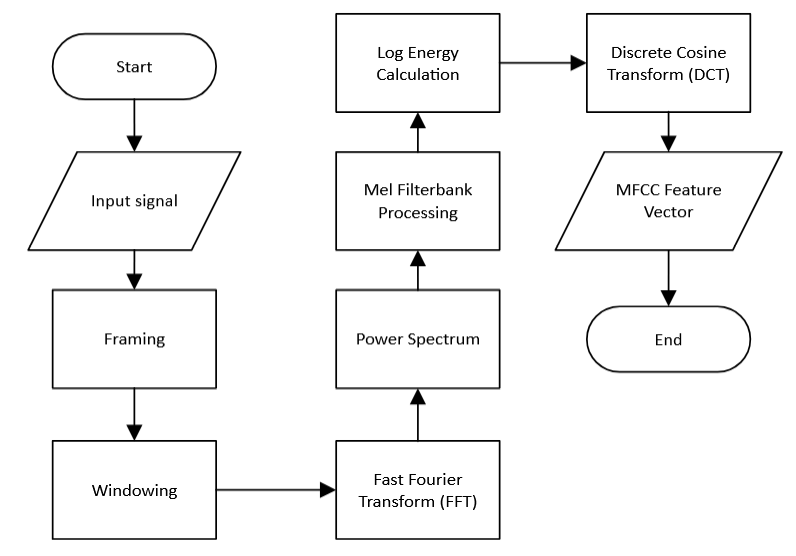
\includegraphics[width=1\linewidth]{img/Audio_feature_extraction_flowchart.png}
  \label{afeflowchart}
  \caption{Audio feature extraction process flowchart}
\end{figure}

\noindent
The audio feature extraction process consists of the following steps (\ref{afeflowchart}):
\begin{enumerate}[nosep]
  \item \textbf{Framing} - Segmenting the signal into short, overlapping frames.
  \item \textbf{Windowing} - Applying a window function to each frame to minimize spectral leakage at the boundaries. The experiments consisted of Hamming window function.
    \end{enumerate}
    \vspace{10pt}
    \[
      w_{\text{Hamming}}[k]=0.54 - 0.46\cos{\left (\frac{2\pi k}{N-1}\right )}
    \]
    \begin{enumerate}[nosep]
  \setcounter{enumi}{2}
  \item \textbf{Fast Fourier Transform (FFT)} - Mapping a time-domain signal into its frequency-domain representation. 
  \[
	A_k=\sum\limits_{p=0}^{n-1}a_pe^{-\dfrac{i2\pi kp}{n}}
  \vspace{-10pt}
    \]
    \vspace{-4pt}
    where:
    \vspace{-3pt}
    \begin{itemize}
      \item $i$ - imaginary unit
      \item $k$ - frequency bin index
      \item $n$ - sample count in frame $a$ (frame length)
      \item $p$ - sample index in the time domain
      \item $a_p$ - sample at index $p$ in frame $a$
    \end{itemize}
  \item \textbf{Power Spectrum} - Computing the energy distribution representation.
  \[
  \tilde{P}_k = \frac{|A_k|^2}{N}
  \]
  where:
    \begin{itemize}
        \item $A_k$ - output of the DFT at frequency bin $k$
        \item $k$ - frequency bin index
        \item $N$ - frame length
        \item $\tilde{P}_k$ - Normalized power spectrum
    \end{itemize}
  \item \textbf{Mel Filterbank Processing} - Constructing a set of triangular filters using Mel scale. This process consists of transferring a vector containing equally distributed Mel-frequency values in the range from $Mel(f_{min})$ to $Mel(f_{max})$ back to Herzian scale to develop the filterbank.
  \[
    Mel(f)=2595\log_{10}\left (1 + \frac{f}{700} \right ) \Rightarrow f=700\cdot10^{\frac{Mel(f)}{2595}-1}
  \]
    where:
    \begin{itemize}
      \item $f$ - frequency in Hz
      \item $Mel(f)$ - frequency in the Mel scale
    \end{itemize}
    
    \[
    	H_m(k)=
    	\begin{cases}
    		0, & k < f_{m-1} \lor k > f_{m+1}\\
    		\dfrac{k-f_{m-1}}{f_{m}-f_{m-1}}, & f_{m-1} \le k \le f_{m}\\
    		\dfrac{f_{m+1}-k}{f_{m+1}-f_{m}}, & f_{m} \le k \le f_{m+1}
    	\end{cases}
	\]
	where:
	\begin{itemize}
		\item $m$ - filter number
		\item $k$ - index of sample frequency
		\item $f$ - vector of filters in Herzian scale
        \item $H$ - Mel filterbank
	\end{itemize}
  \item \textbf{Log Energy Calculation} - Mapping the linear frequency spectrum to Mel scale using Mel filterbank.
  \[
    S_m^{log}=\log_{10}\left (\sum\limits_k P_k\cdot H_m(k)\right )
  \]
  \item \textbf{Discrete Cosine Transform (DCT)} - Decorrelating the log energies to get Mel-Frequency Cepstral Coefficients
  \[
	c_m=\sum\limits^{k-1}_{p=0}S_m^{log}\cdot \cos{\left (\dfrac{\pi m(p+0.5)}{k}\right )}
	\]
	where:
	\begin{itemize}
		\item m - Mel coefficient index
		\item k - Chosen count of Mel coefficients
        \item c - Mel coefficient vector
	\end{itemize}
\end{enumerate}

\subsection{Machine Learning Algorithms}

\subsubsection{Random Forest}

The Random Forest algorithm was chosen for classification purposes, a well-known ensemble learning method originally introduced by Leo Breiman \cite{breiman2001random}. Essentially, instead of relying on just one model, it constructs a whole bunch of individual decision trees during the training phase and aggregates their predictions to get the final output. Since we are dealing with classification, the model determines the final predicted class by running a majority vote across all the trees in the forest:

\begin{equation}
	\hat{y} = \arg\max_{c} \sum_{t=1}^{T} \mathbf{1}\left[h_t(\mathbf{x}) = c\right]
\end{equation}

\noindent In this equation, $T$ stands for the total number of trees, $h_{t}(x)$ is the prediction made by the $t$-th tree for our input $x$, and $c$ represents the possible classes we are trying to predict.\\

\noindent To make the ensemble robust and prevent the trees from being too similar, each tree is trained on what is called a "bootstrap sample"—basically, a random subset of our training data selected with replacement. On top of that, when splitting a node, the algorithm doesn't look at all available features at once. Instead, it only considers a random subset of $m$ features out of the total $p$ features. This clever trick decorrelates the individual trees, which drastically cuts down the overall variance of the model \cite{breiman2001random}.\\

\noindent To pick the best possible split at any given node, the algorithm evaluates how "pure" the resulting splits will be by minimizing the Gini impurity:

\begin{equation}
	G(S) = 1 - \sum_{c=1}^{C} p_c^2
\end{equation}

\noindent Here, $S$ is the set of samples currently at the node, $C$ represents the number of classes, and $p_{c}$ is the proportion of samples belonging to class $c$. The actual split into left ($S_{L}$) and right ($S_{R}$) subsets is chosen to maximize the information gain ($\Delta G$):

\begin{equation}
	\Delta G = G(S) - \frac{|S_L|}{|S|} G(S_L) - \frac{|S_R|}{|S|} G(S_R)
\end{equation}

\noindent One of the biggest practical advantages of using Random Forests is something called the out-of-bag (OOB) error estimate. Because of how the bootstrap sampling works, roughly 36.8\% of the training data is left out of any single tree's training process on average. We can actually use these left-out samples as an internal validation set. This has a couple of advantages an unbiased estimate of how well our model generalizes without needing to sacrifice data for a separate validation split \cite{breiman2001random}:

\begin{equation}
	\text{OOB Error} = \frac{1}{N} \sum_{i=1}^{N} \mathbf{1}\left[\hat{y}_i^{\text{OOB}} \neq y_i\right]
\end{equation}

\noindent In this formula, $\hat{y}_{i}^{OOB}$ is the majority vote prediction for sample $i$ using only the specific trees that did not see this sample during their training, and $N$ is the total number of training samples.\\

\noindent When it comes to classifying bird species from MFCC data, Random Forest gives us a couple of great advantages: its built-in feature importance scores make it easy to identify which spectral coefficients actually matter, and its ensemble structure keeps it from getting easily thrown off by noisy or irrelevant audio features \cite{huang2024recognition, ahmed2023bird}.

\subsubsection{Neural Network}

\hl{do uzupelnienia}
\newpage

\section{Experiments}
\hl{brakuje opisu zbioru danych, podzialu danych, jak również informacji o wykorzystanym sprzecie do obliczeń}

\subsection{Audio Feature Extraction}

To analyse the MFCC efficiency based on the number of Mel filters and extracted features the experiments were conducted on dataset which was reduced to 1148 records. Both the Random Forest and the Neural Network were applied to check the F1 score for every configuration.
\vspace{-5pt}
\begin{figure}[htbp]
  \centering
  \begin{subfigure}{0.4665\linewidth}
    \centering
    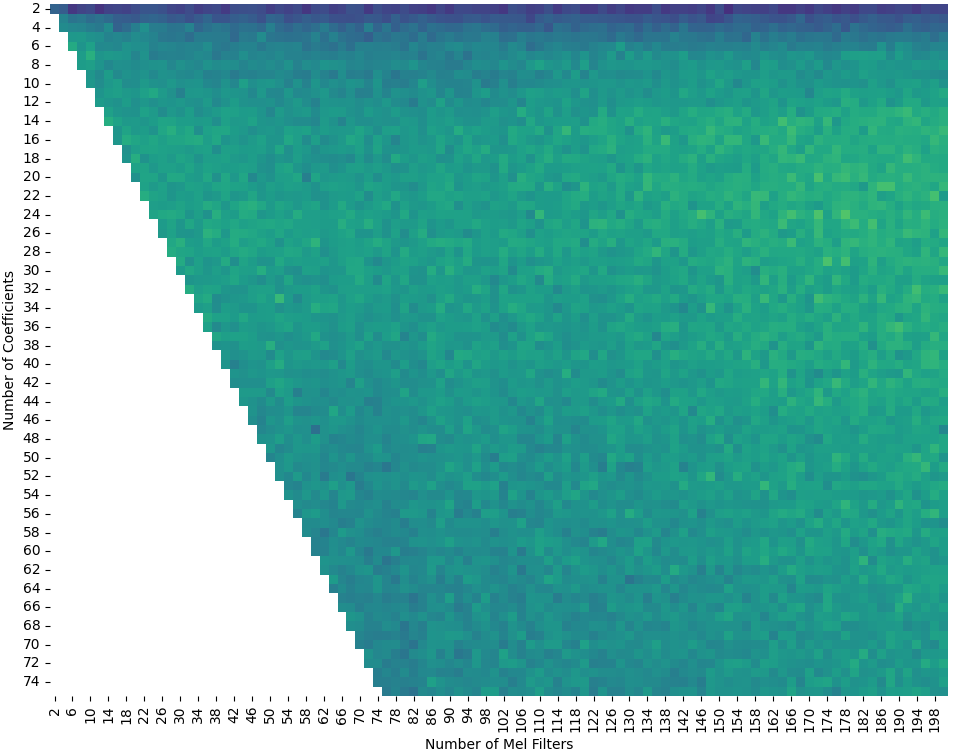
\includegraphics[width=\linewidth]{img/rf_results_if0.png}
    \caption{Dataset with every coefficient}
  \end{subfigure}
  \begin{subfigure}{0.524\linewidth}
    \centering
    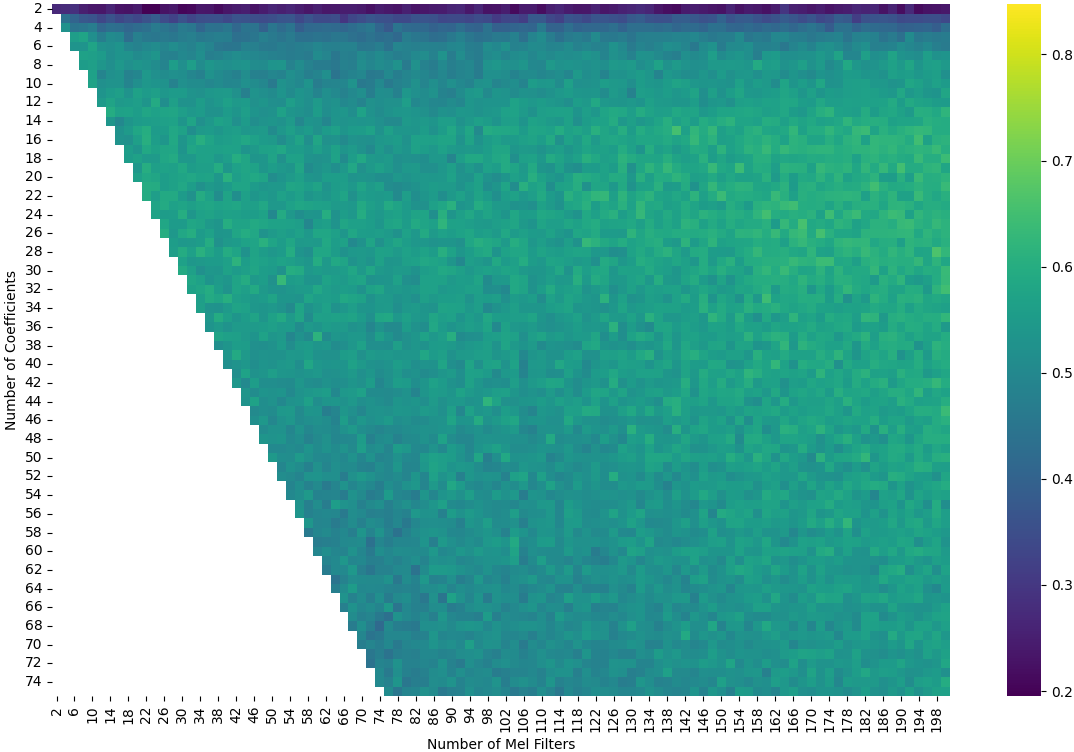
\includegraphics[width=\linewidth]{img/rf_results_if1.png}
    \caption{Dataset without first coefficient}
  \end{subfigure}
  \caption{Random Forest F1 Score heatmaps for datasets with and without first coefficient}
  \label{rfhm}
\end{figure}

\vspace{-27pt}
\begin{center}
\rule{0.9\linewidth}{1pt}
\end{center}
\vspace{-20pt}

\begin{figure}[htbp]
  \centering
  \begin{subfigure}[b]{0.4665\linewidth}
    \centering
    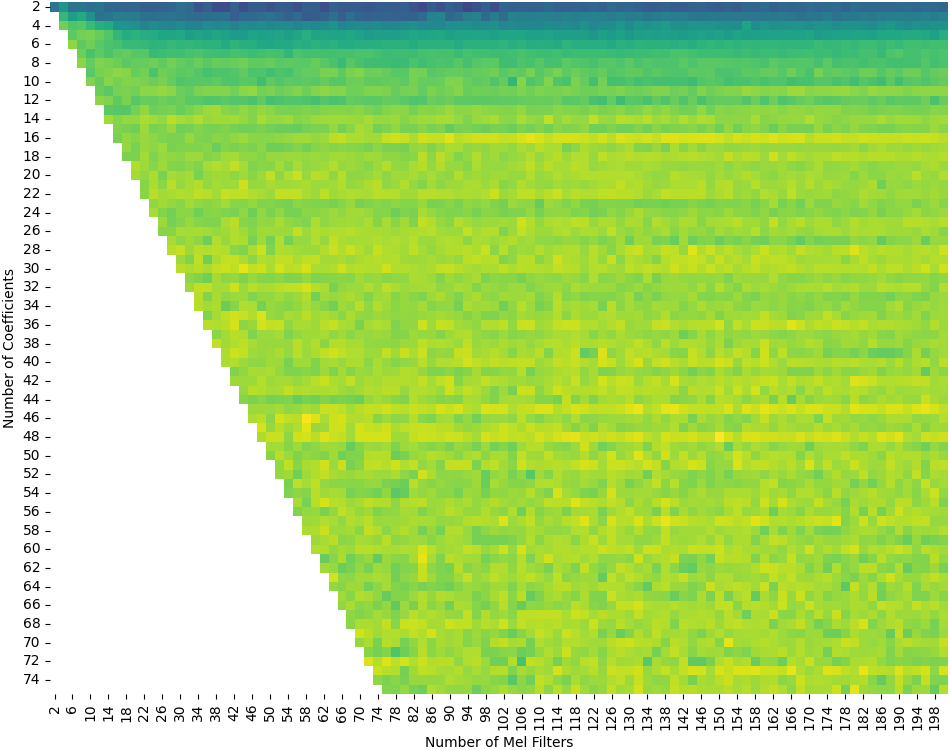
\includegraphics[width=\linewidth]{img/nn_results_if0.png}
    \caption{Dataset with every coefficient}
  \end{subfigure}
  \begin{subfigure}[b]{0.524\linewidth}
    \centering
    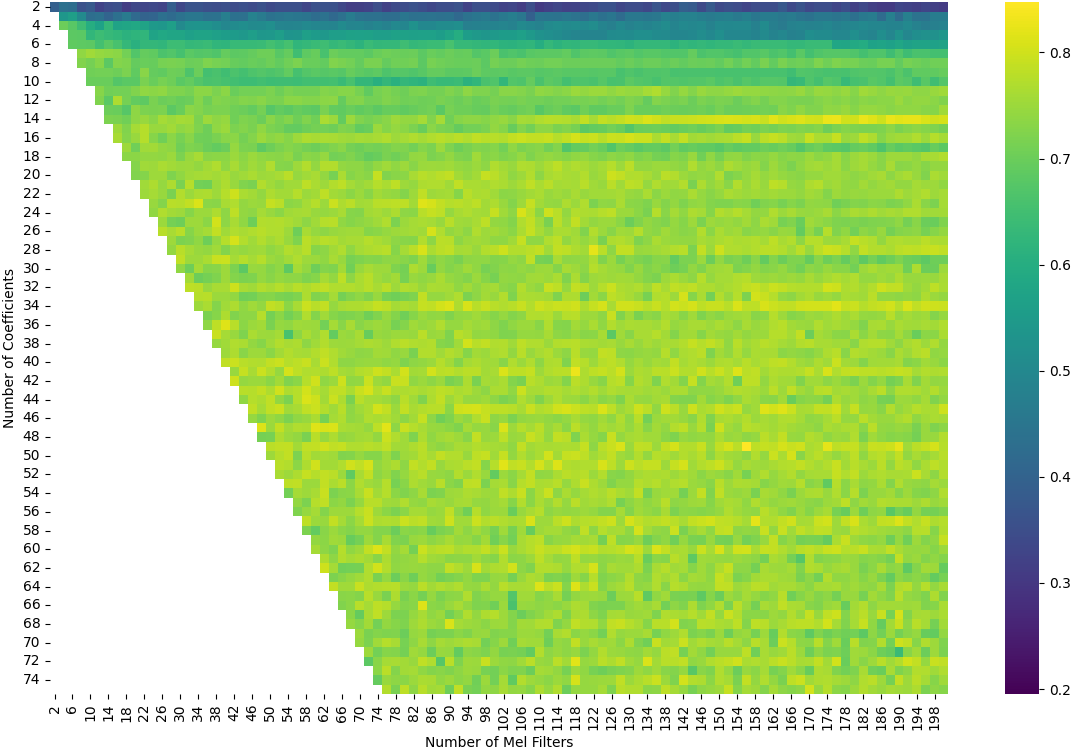
\includegraphics[width=\linewidth]{img/nn_results_if1.png}
    \caption{Dataset without first coefficient}
  \end{subfigure}
  \caption{Neural Network F1 Score heatmaps for datasets with and without first coefficient}
  \label{nnhm}
\end{figure}

\vspace{-30pt}
\begin{center}
\rule{0.9\linewidth}{1pt}
\end{center}
\vspace{-20pt}

\begin{figure}[htbp]
  \centering
  \caption{Best results}
  \begin{tabular}{|c|c|c|c|c|}
    \hline
    Algorithm & N Coefficients & N Filters & First Coefficient Ignored & F1 Score \\\hline
    Random Forest & 24 & 178 & No & 0.6669 \\\hline
    Random Forest & 28 & 198 & Yes & 0.6618 \\\hline
    Neural Network & 48 & 150 & No & 0.8472 \\\hline
    Neural Network & 49 & 156 & Yes & 0.8454 \\\hline
  \end{tabular}
  \label{br}
\end{figure}
\vspace{20pt}
\noindent
While standard speech recognition systems typically employ 13 Mel coefficients and between 26 and 40 Mel filters\cite{joshi2014matlab,mahmood2021speech,al2023mel}, our results demonstrate that bird species identification requires a higher spectral resolution. The optimal configuration for the Neural Network was observed in the range of 45-49 Mel coefficients with at least 58 Mel filters (\ref{nnhm}), whereas the Random Forest achieved its best performance with 21-25 Mel coefficients and at least 146 Mel filters (\ref{rfhm}). These results emphasize the fact that birdsong contains faster frequency modulations and more complex harmonic structures compared to human speech, requiring a denser filterbank to effectively capture significant parts of the sound, which is essential for accurate species discrimination. Both machine learning algorithms achieved higher results analysing every coefficient, including the first one, which represents the volume. The first coefficient often reaches massive values, dominating other coefficients and making machine learning performance dependent on the distance of microphone. However, experiments have shown, that including this coefficient in examined dataset actually improves the efficiency (\ref{br}).
\\
The difference in the optimal spectral resolutions between the two models highlights the higher sensitivity of the Random Forest to excessive feature counts, which can degrade its performance. In contrast, the Neural Network effectively manages high-dimensional inputs, achieving better performance by capturing more complex patterns within the given data.
\subsection{Random Forest}
\subsection{Neural Network}

\hl{proszę dodać ajką analizę innych metryk typu accuracy, error, analizę sieci neuronowej - ile warstw, dlaczego, co jesli sie zmniejszy ta ilosc itd.}


\section{Conclusion}
\hl{do uzupelnienia}

\bibliography{bibliography}

\end{document}